\documentclass[a4paper, 12pt]{article}%тип документа

%отступы
\usepackage[left=2cm,right=2cm,top=2cm,bottom=3cm,bindingoffset=0cm]{geometry}

%Русский язык
\usepackage[T2A]{fontenc} %кодировка
\usepackage[utf8]{inputenc} %кодировка исходного кода
\usepackage[english,russian]{babel} %локализация и переносы

%Вставка картинок
\usepackage{wrapfig}
\usepackage{graphicx}
\graphicspath{{pictures/}}
\DeclareGraphicsExtensions{.pdf,.png,.jpg}

%оглавление
\usepackage{titlesec}
\titlespacing{\chapter}{0pt}{-30pt}{12pt}
\titlespacing{\section}{\parindent}{5mm}{5mm}
\titlespacing{\subsection}{\parindent}{5mm}{5mm}
\usepackage{setspace}

%Графики
\usepackage{multirow}
\usepackage{pgfplots}
\pgfplotsset{compat=1.9}

%Математика
\usepackage{amsmath, amsfonts, amssymb, amsthm, mathtools}

%Заголовок
\author{Сорокин Вадим\\
828 группа}
\title{\textbf{Работа Д4.2\\
Изучение закона поглощения в жидкости}}
\date{}
\newtheorem{task}{Задача}
\begin{document}
\maketitle
\subsection*{Цель работы}
экспериментально проверить закон Ламберта-Бугера-Бера и измерить коэффициент поглощения крепкого чайного настоя.
\subsection*{Оборудование}
Настольная лампа, высокий стакан, линейка, черная бумага, настой чайных листьев, белая крышка, тонкий стержень, штатив, фотоаппарат, компьютер.
\section*{Теория}
Молекулы веществ способны поглощать световую энергию на определенных частотах. Спектр поглощения различен. Однако можно утверждать, что ослабление интенсивности будет пропорционально количеству молекул, провзаимодействовавших со светом. Пусть р – вероятность поглощения фотона молекулой, тогда при взаимодействии с N молекулами, число фотонов уменьшится на
\[dN_{\text{ф}} = - p N_{\text{ф}}dN\]
где $p$ --- вероятность поглощения фотона молекулой.
Пусть световой поток падает на плоский слой поглощающего вещества толщиной $dx$ перпендикулярно его поверхности площадью $S$. Если обозначить концентрацию молекул в слое как $n$, то $N = nSdx$. Таким образом, скорость изменения интенсивности пропорциональна интенсивности 
\[dI =-\alpha I dx\]
Проинтегрировав это выражение, получим закон Ламберта-Бугера-Бера 
\[I = I_0e^{-\alpha x}\]
где $I_0$ --- интенсивность падающего на поглощающую среду света ($x = 0$), $\alpha$ --- коэффициент поглощения, $x$ --- длина пути света в поглощающей среде.
\section*{Схема установки}
В стакан, заполненный исследуемой жидкостью и обёрнутый чёрной бумагой, на глубину h помещается белый пластмассовый диск на держателе Д. Сверху диск освещаем с помощью источника Л и делаем фотоснимок с помощью камеры Ф. Затем снимок анализируем и получаем $I$. 
\begin{figure}[h]
\begin{center}
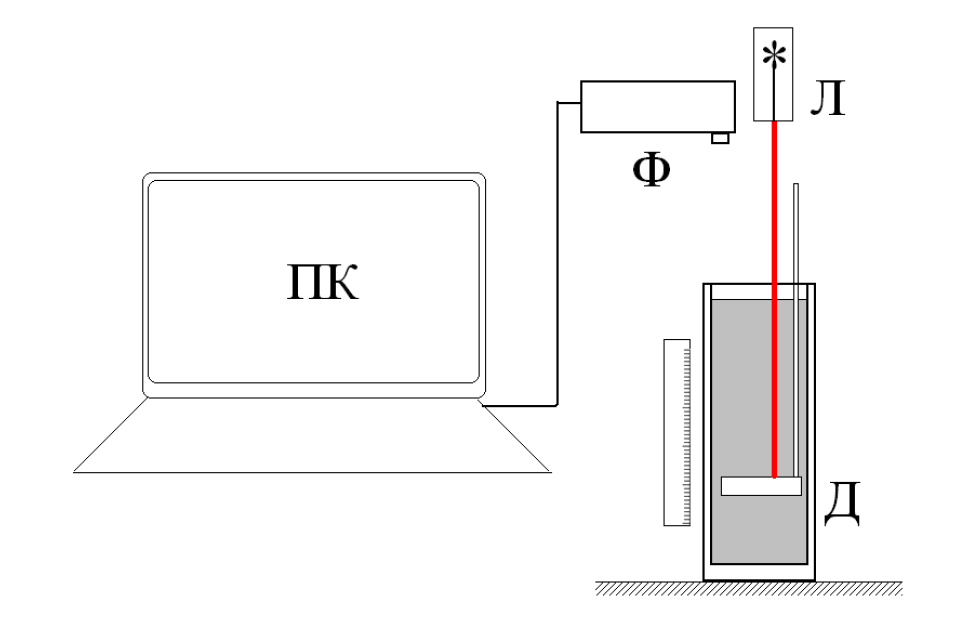
\includegraphics[width = 0.4\textwidth]{4.png}
\caption{Схема установки}
\end{center}
\end{figure}
В данной работе используем экспериментальную установку, показанную на фото, для уменьшения погрешностей постоянно фокусируем телефон на центр стакана
\begin{figure}[h]
\begin{center}
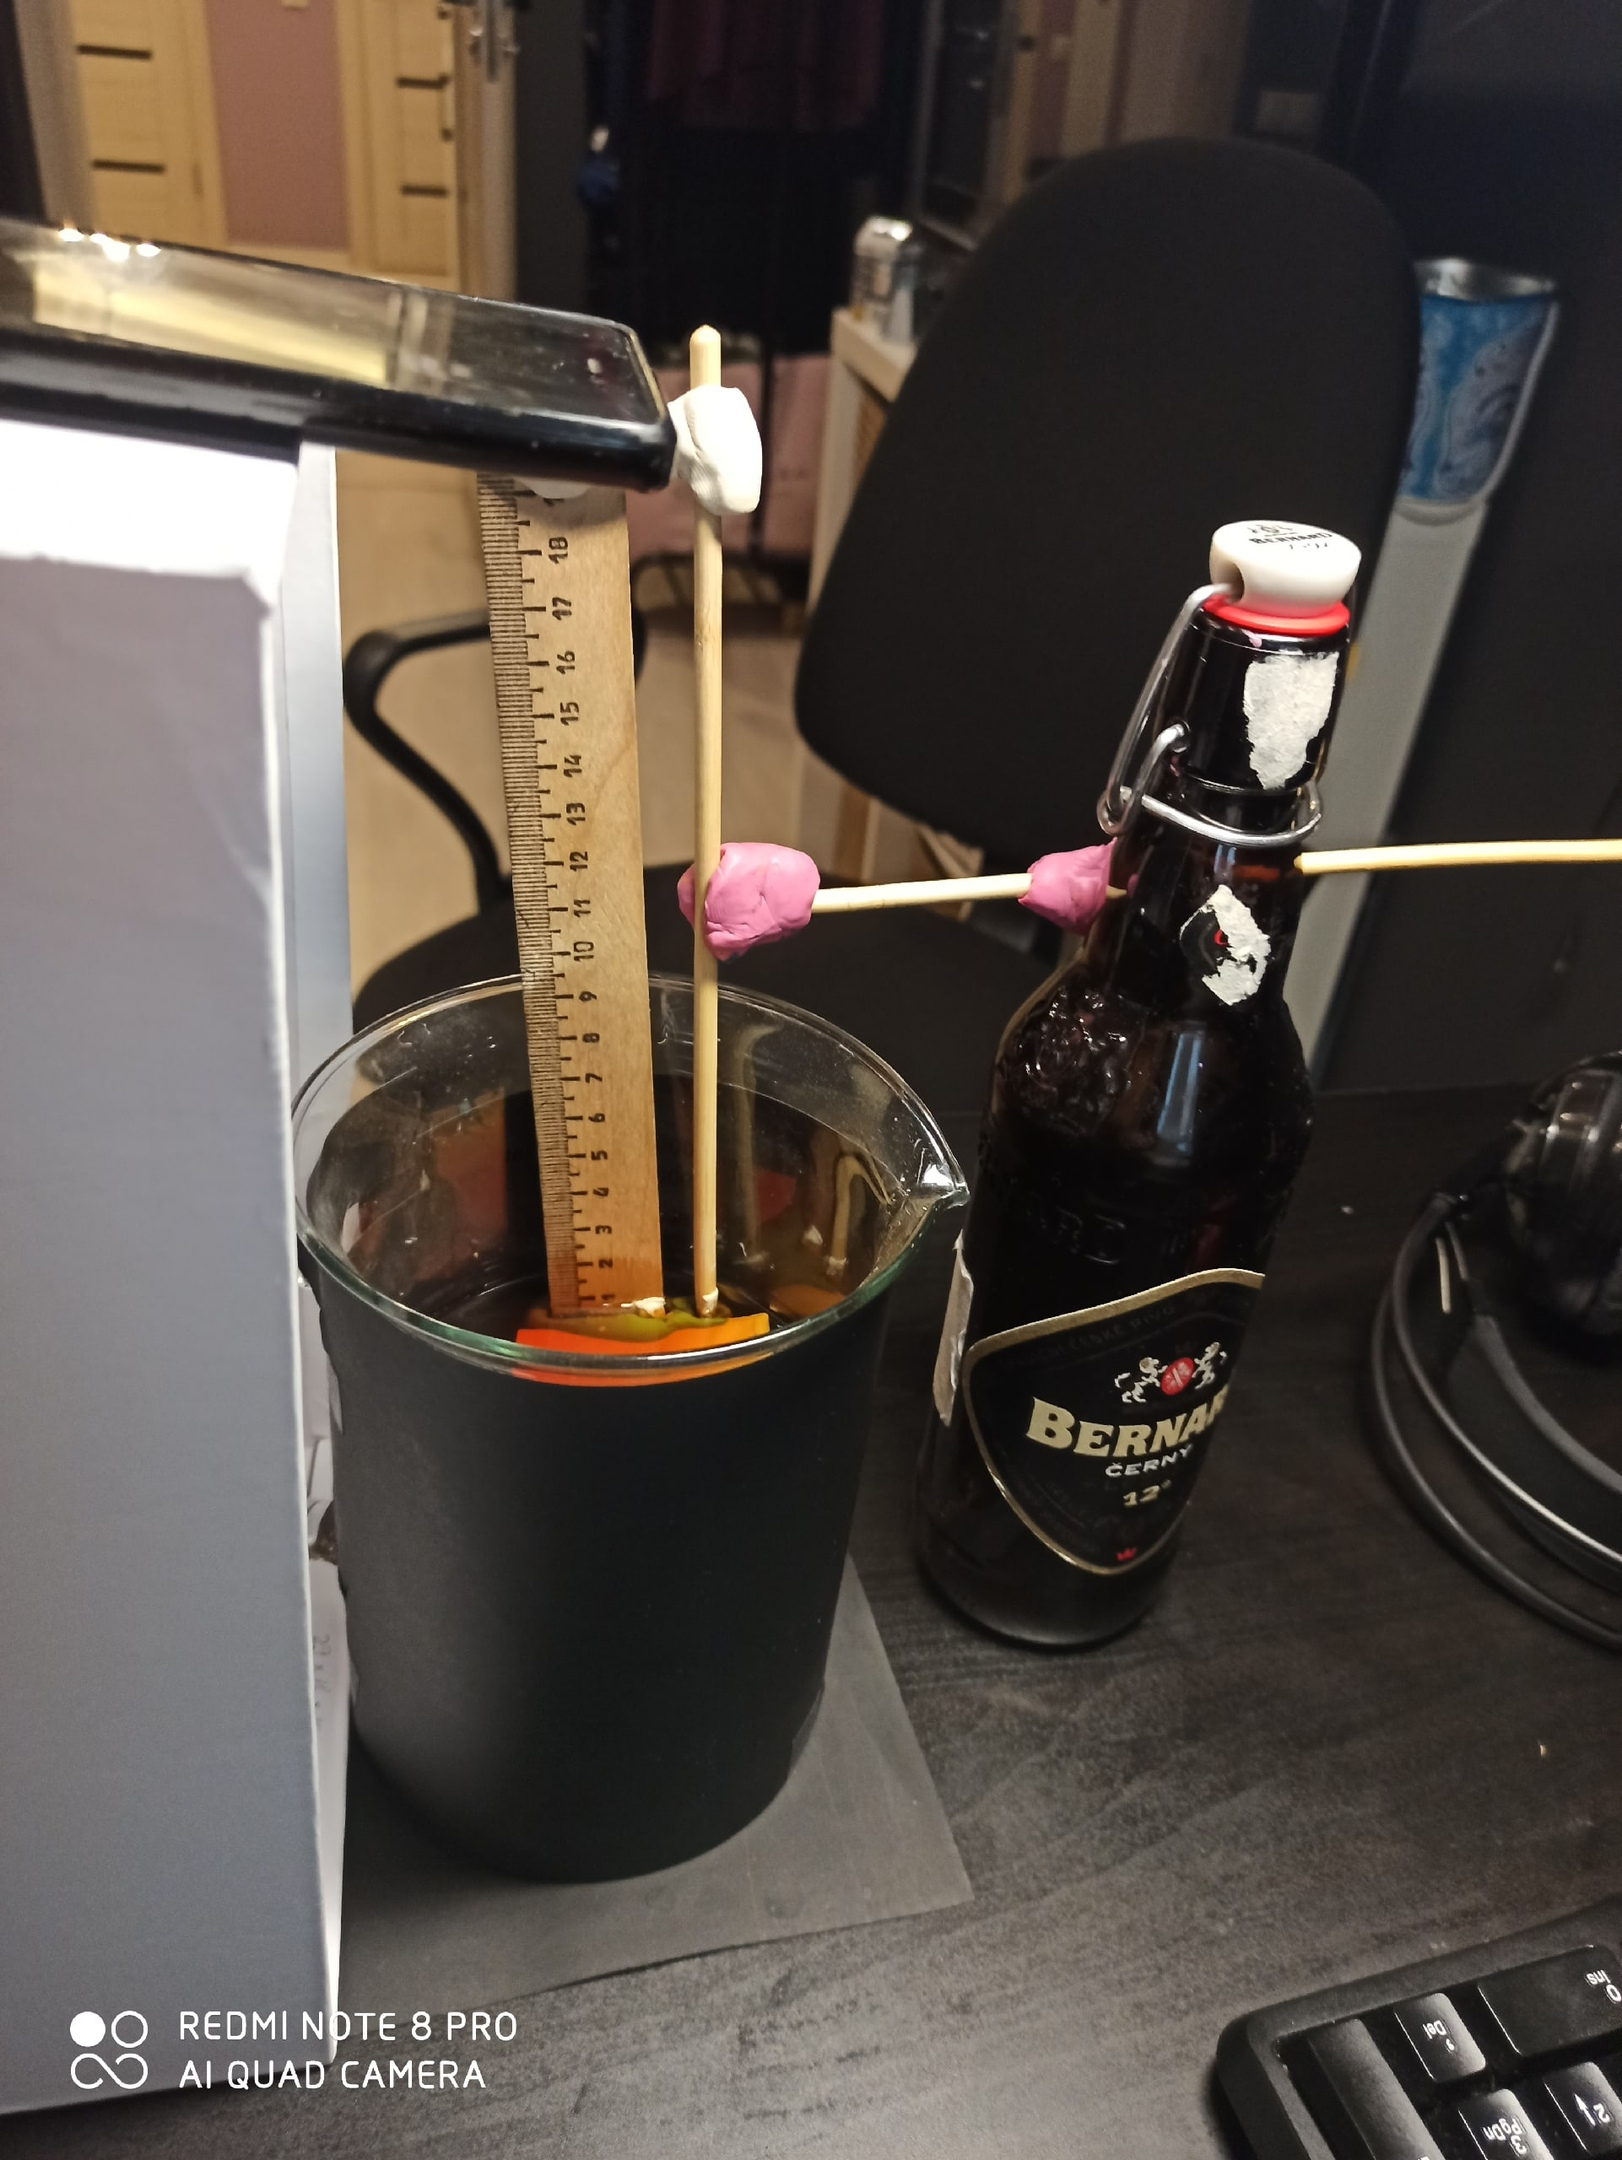
\includegraphics[width = 0.4\textwidth]{3.jpg}
\caption{Фотография установки}
\end{center}
\end{figure}
\section*{Ход работы}
\subsection*{Определение поглощения воды}
Для этого проведем эксперимент, измеряя яркость в зависимости от глубины погружения в воду, которую мы определим по линейке. примем погрешность линейки за 1 см, поскольку видно, что нам лучше всего определять глубину с точностью до 1 см, то есть по большим рискам на линейке. Считаем яркость по квадрату в центре 10х10, поскольку сам диск немного неровный, и считаем среднее яркости в программе. Погрешность для $I$ считаем по формуле
\[\delta I = \frac{1}{\sqrt{100\cdot99}}\sqrt{\sum\limits_{i = 1}^{100} \left(I_i - \overline{I}\right)^2}\]
Все данные занесем в таблицу 1.

\begin{table}[h]
\begin{center}
\begin{tabular}{|c|c|c|c|c|c|}
\hline
$h$, см & $\delta_h$, см & $I$, у.е. & $\delta_I$, у.е. & $\ln(I/I_0)$ & $\delta_{\ln(I/I_0)}$ \\ \hline
0       & 1              & 500       & 70               & 0            & 0                     \\ \hline
2       & 1              & 470       & 70               & -0,06        & 0,01                  \\ \hline
4       & 1              & 460       & 60               & -0,08        & 0,02                  \\ \hline
6       & 1              & 460       & 60               & -0,08        & 0,02                  \\ \hline
8       & 1              & 460       & 60               & -0,08        & 0,02                  \\ \hline
10      & 1              & 440       & 60               & -0,12        & 0,02                  \\ \hline
12      & 1              & 420       & 50               & -0,17        & 0,03                  \\ \hline
14      & 1              & 420       & 50               & -0,17        & 0,03                  \\ \hline
16      & 1              & 400       & 50               & -0,22        & 0,04                  \\ \hline
18      & 1              & 400       & 50               & -0,22        & 0,04                  \\ \hline
20      & 1              & 390       & 50               & -0,24        & 0,04                  \\ \hline
\end{tabular}
\caption{Зависимость $I(h)$ для воды}
\end{center}
\end{table}
Далее строим график зависимости, аппроксимируем и считаем погрешность по МНК. 

\begin{figure}[h]
\begin{center}
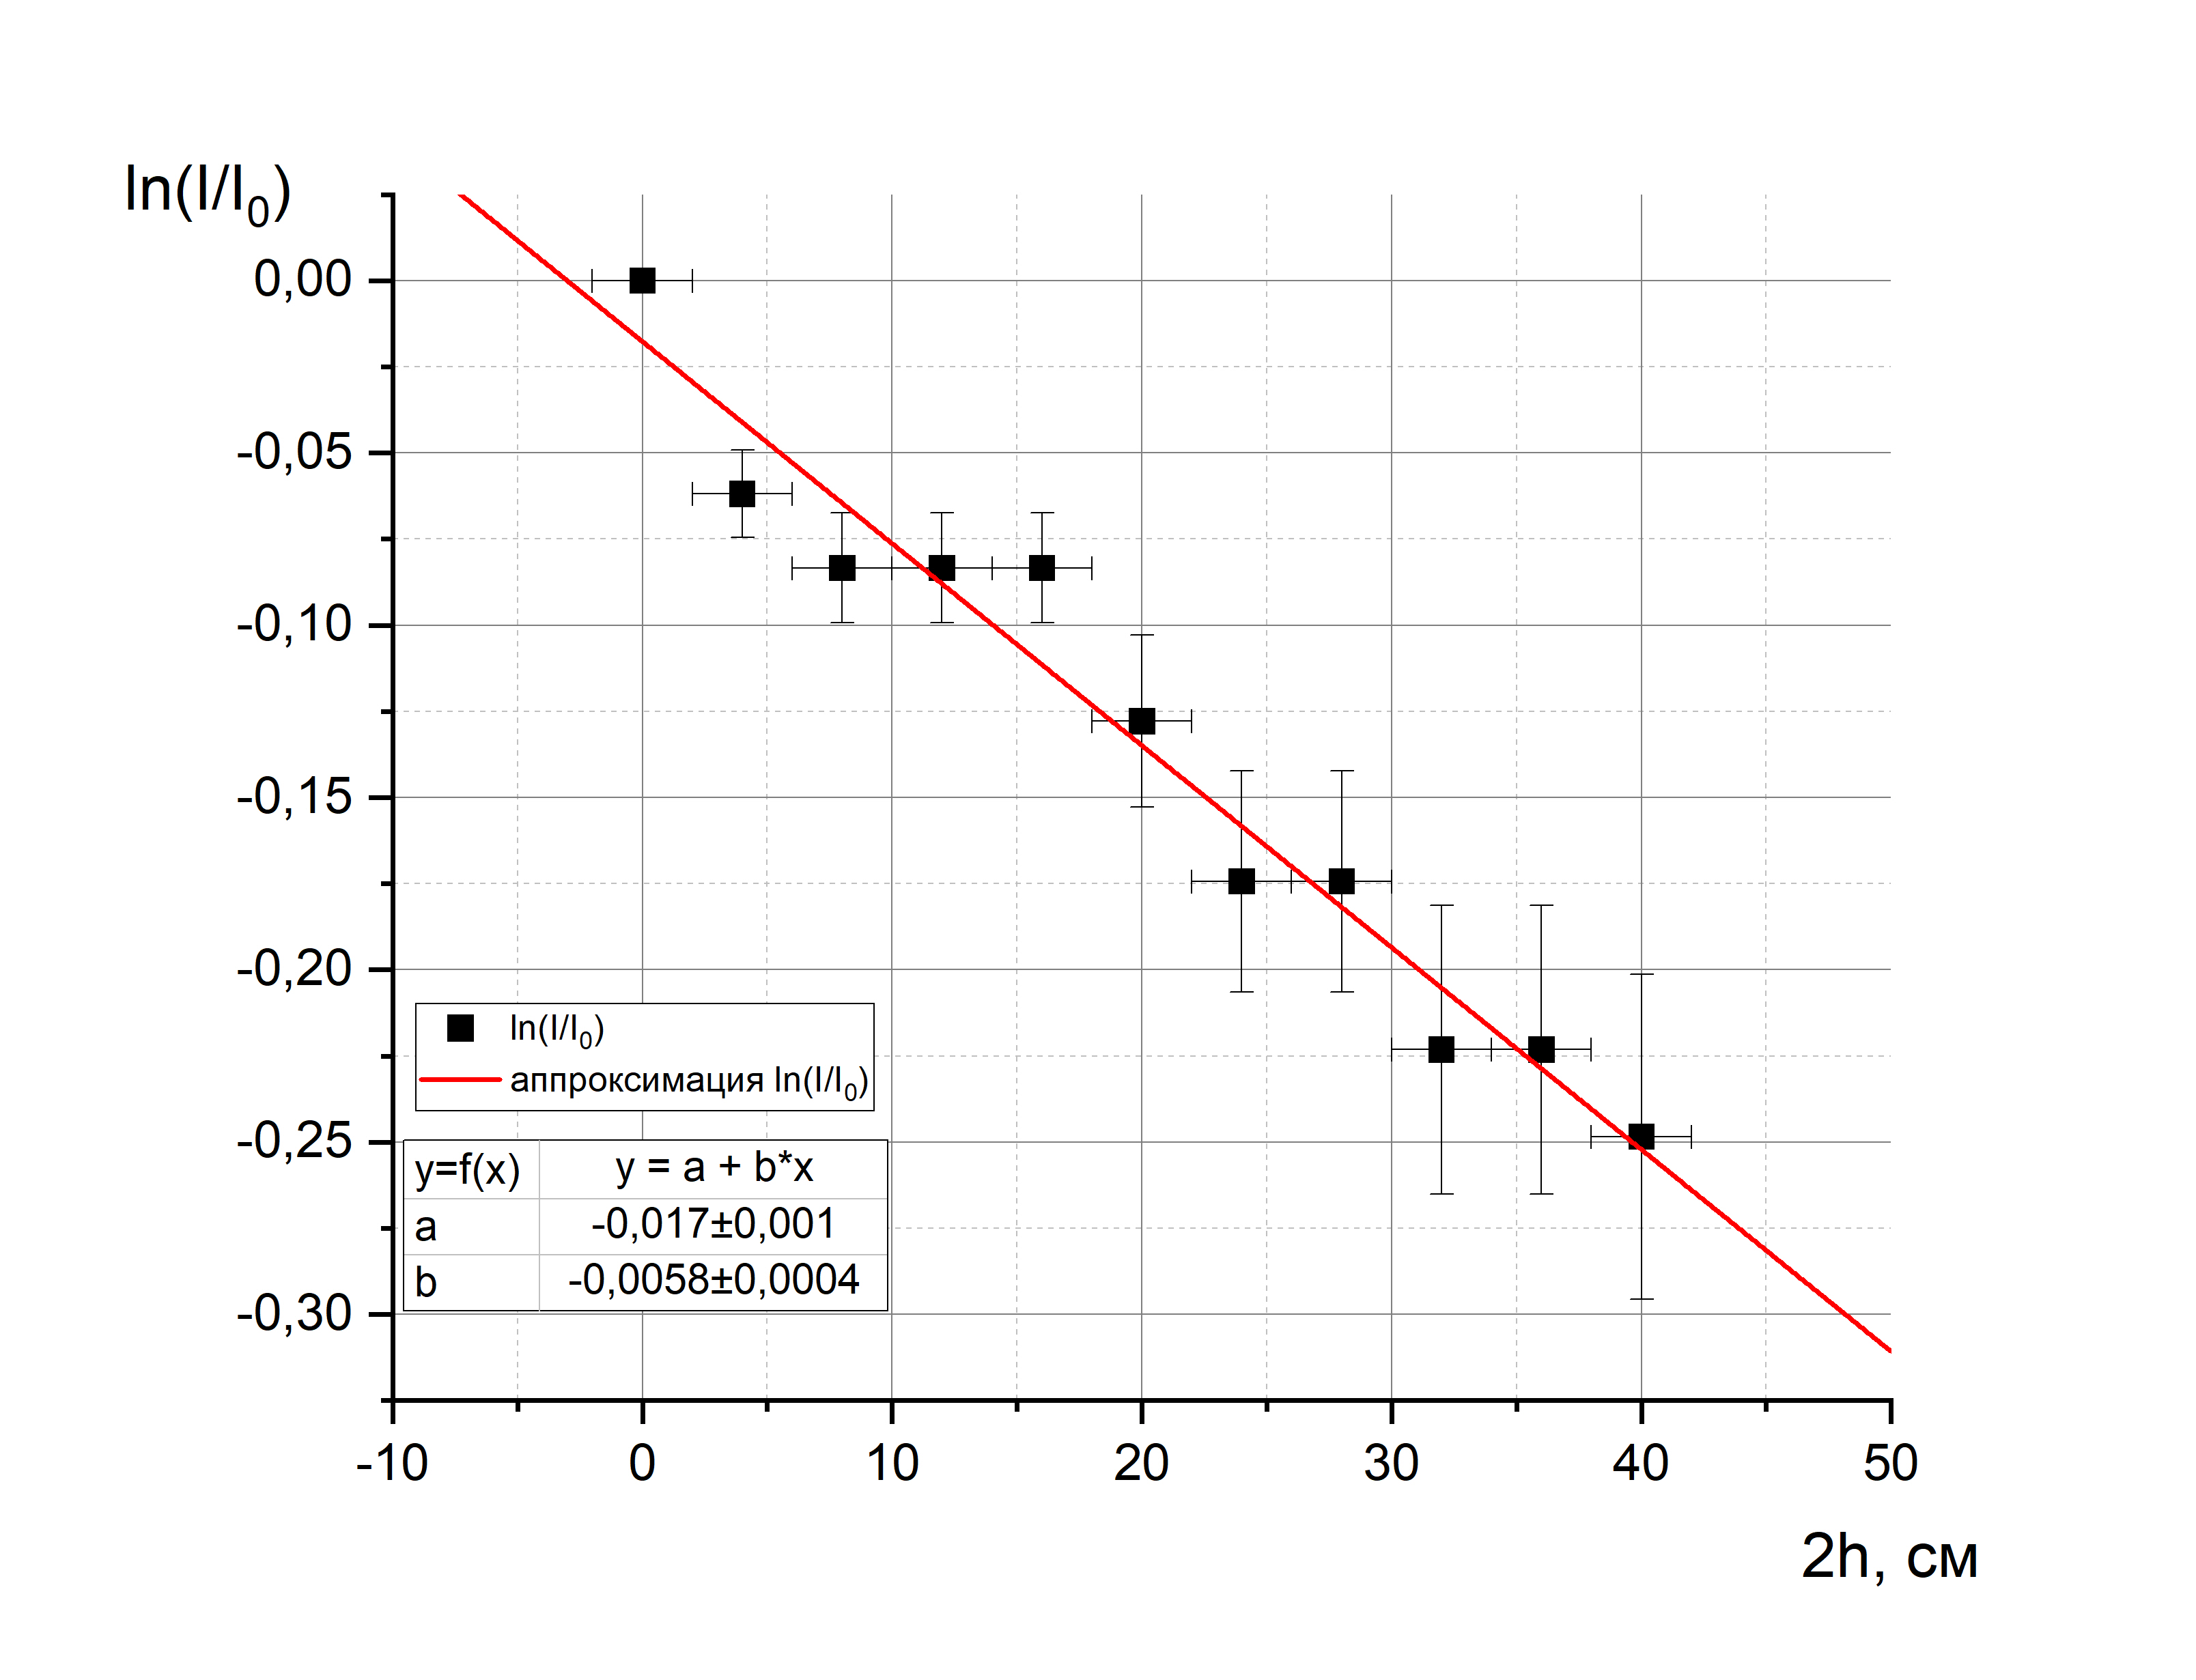
\includegraphics[width = 0.7\textwidth]{1.jpg}
\caption{График зависимости $ln(I/I_0) (2h)$ для воды }
\end{center}
\end{figure}
В итоге получаем, что 
\[\alpha_{water} = (0,58 \pm 0,04) \text{м}^{-1}\]
\newpage
\subsection*{Определение поглощения чая}
Делаем все то же самое, что и для воды
\begin{table}[h]
\begin{center}

\begin{tabular}{|c|c|l|c|c|c|}
\hline
$h$, см & $\delta_h$, см & $I$, у.е. & $\delta_I$, у.е. & $\ln(I/I_0)$ & $\delta_{\ln(I/I_0)}$ \\ \hline
0       & 1              & 500       & 70               & 0            & 0                     \\ \hline
2       & 1              & 340       & 60               & -0,4         & 0,1                   \\ \hline
4       & 1              & 220       & 50               & -0,8         & 0,2                   \\ \hline
6       & 1              & 170       & 30               & -1,1         & 0,2                   \\ \hline
8       & 1              & 100       & 20               & -1,6         & 0,4                   \\ \hline
10      & 1              & 70        & 20               & -2           & 0,6                   \\ \hline
12      & 1              & 40        & 10               & -2,5         & 0,7                   \\ \hline
14      & 1              & 30        & 10               & -3           & 1                     \\ \hline
16      & 1              & 20        & 5                & -3,2         & 0,9                   \\ \hline
18      & 1              & 10        & 2                & -4           & 1                     \\ \hline
20      & 1              & 10        & 2                & -4           & 1                     \\ \hline
\end{tabular}
\caption{Зависимость $I(h)$ для чая}
\end{center}
\end{table}
\begin{figure}[h]
\begin{center}
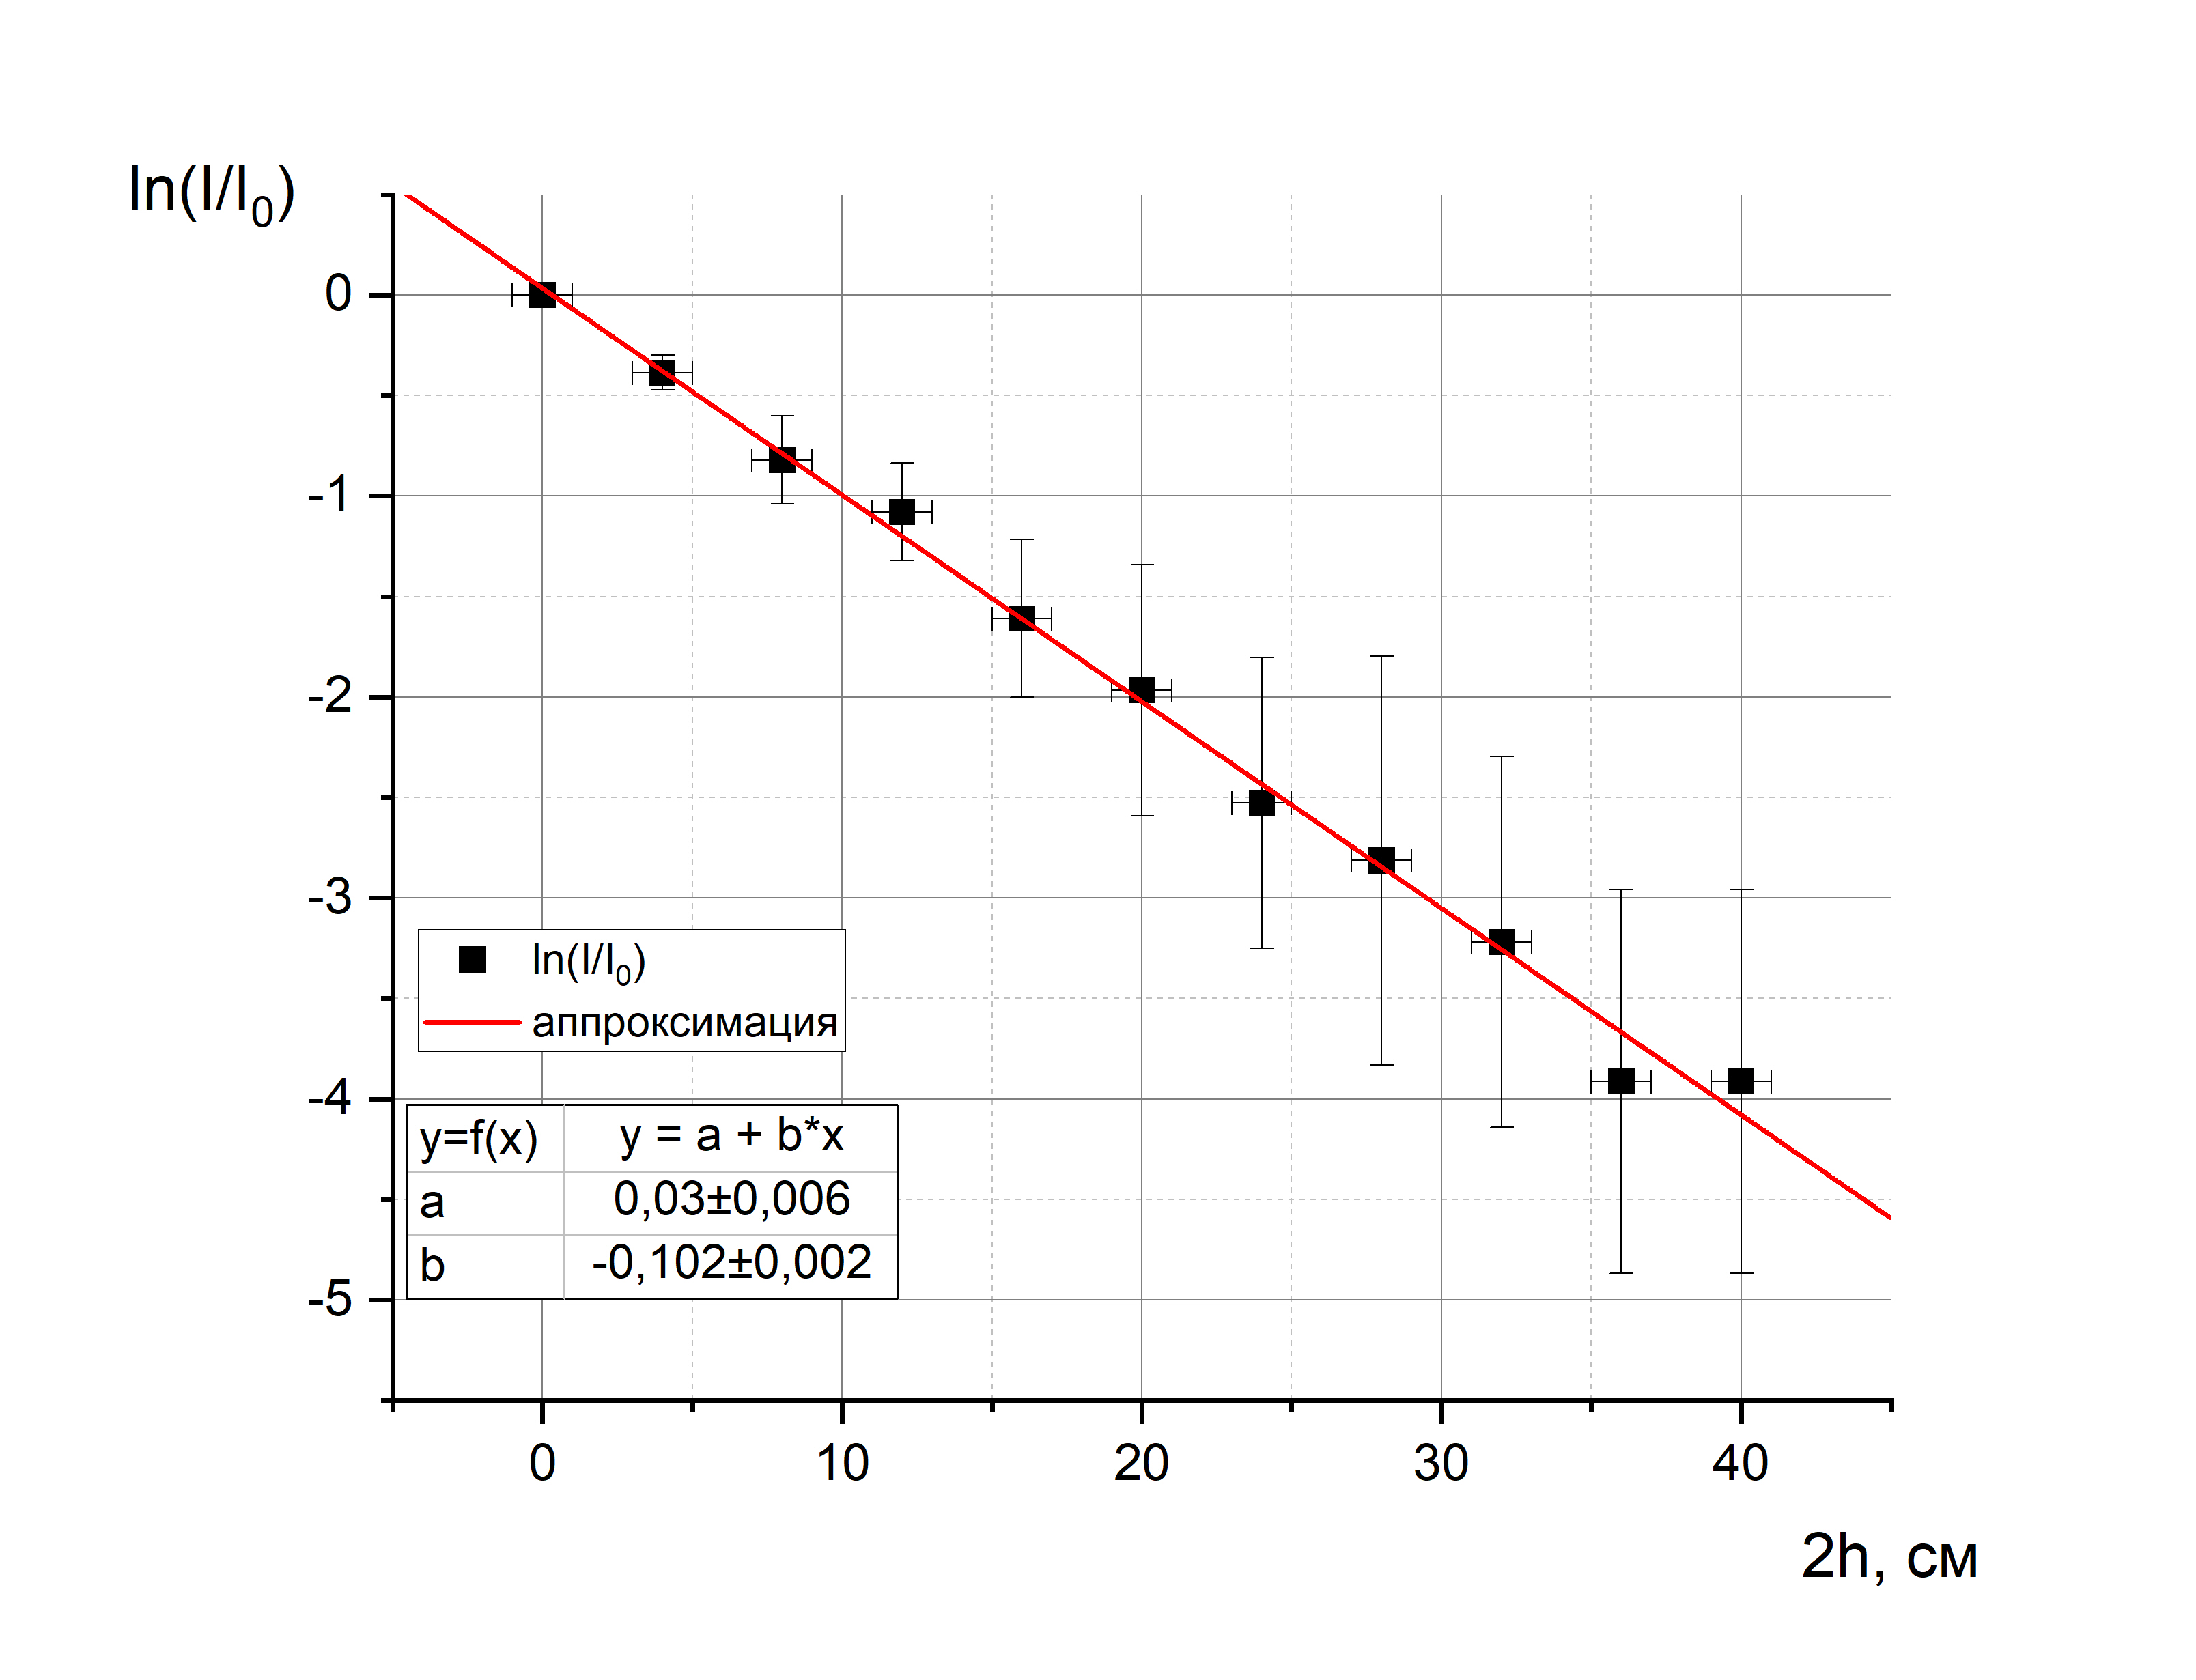
\includegraphics[width = 0.7\textwidth]{2.jpg}
\caption{График зависимости $ln(I/I_0) (2h)$ для чая }
\end{center}
\end{figure}

В итоге получаем, что для чая $\alpha_{tea} = (10,2 \pm 0,2)\text{м}^{-1}$
\newpage
\subsection*{Измерение относительной концентрации поглощающих веществ}
Для этого будем класть чай в холодную воду, чтобы успеть хоть что-то зафиксировать, естественно для этого опыта придется пожертвовать точность, и делать меньше измерений при каждой "времени". Все остальное делаем как и для чая и для воды. Все данные заносим в таблицу. 

\begin{table}[h]
\begin{center}

\begin{tabular}{|c|c|c|c|c|c|}
\hline
\multicolumn{6}{|c|}{t=5мин}                                                                   \\ \hline
$h$, см & $\delta_h$, см & $I$, у.е. & $\delta_I$, у.е. & $\ln(I/I_0)$ & $\delta_{\ln(I/I_0)}$ \\ \hline
0       & 1              & 490       & 70               & 0,00         & 0,00                  \\ \hline
4       & 1              & 440       & 70               & -0,11        & 0,02                  \\ \hline
8       & 1              & 390       & 60               & -0,23        & 0,05                  \\ \hline
12      & 1              & 340       & 60               & -0,37        & 0,08                  \\ \hline
16      & 1              & 300       & 50               & -0,5         & 0,1                   \\ \hline
20      & 1              & 280       & 50               & -0,6         & 0,1                   \\ \hline
\multicolumn{6}{|c|}{t=50мин}                                                                  \\ \hline
$h$, см & $\delta_h$, см & $I$, у.е. & $\delta_I$, у.е. & $\ln(I/I_0)$ & $\delta_{\ln(I/I_0)}$ \\ \hline
0       & 1              & 500       & 70               & 0,00         & 0,00                  \\ \hline
4       & 1              & 410       & 60               & -0,20        & 0,04                  \\ \hline
8       & 1              & 330       & 50               & -0,42        & 0,09                  \\ \hline
12      & 1              & 270       & 50               & -0,6         & 0,1                   \\ \hline
16      & 1              & 230       & 40               & -0,8         & 0,2                   \\ \hline
20      & 1              & 180       & 40               & -1,0         & 0,3                   \\ \hline
\multicolumn{6}{|c|}{t=100мин}                                                                 \\ \hline
$h$, см & $\delta_h$, см & $I$, у.е. & $\delta_I$, у.е. & $\ln(I/I_0)$ & $\delta_{\ln(I/I_0)}$ \\ \hline
0       & 1              & 490       & 70               & 0,00         & 0,00                  \\ \hline
4       & 1              & 380       & 60               & -0,25        & 0,05                  \\ \hline
8       & 1              & 300       & 50               & -0,5         & 0,1                   \\ \hline
12      & 1              & 220       & 50               & -0,8         & 0,2                   \\ \hline
16      & 1              & 160       & 40               & -1,1         & 0,3                   \\ \hline
20      & 1              & 140       & 30               & -1,3         & 0,3                   \\ \hline
\multicolumn{6}{|c|}{t=2000мин}                                                                \\ \hline
$h$, см & $\delta_h$, см & $I$, у.е. & $\delta_I$, у.е. & $\ln(I/I_0)$ & $\delta_{\ln(I/I_0)}$ \\ \hline
0       & 1              & 500       & 70               & 0,00         & 0                     \\ \hline
4       & 1              & 220       & 50               & -0,8         & 0,2                   \\ \hline
8       & 1              & 100       & 20               & -1,6         & 0,4                   \\ \hline
12      & 1              & 40        & 10               & -2,5         & 0,7                   \\ \hline
16      & 1              & 20        & 5                & -3,2         & 0,9                   \\ \hline
20      & 1              & 10        & 2                & -3,9         & 1,0                   \\ \hline
\end{tabular}
\caption{Данные зависимости $I(h)$ для чая при различном времени заварки}	
\end{center}
\end{table}
\newpage
\begin{figure}[h]
\begin{center}
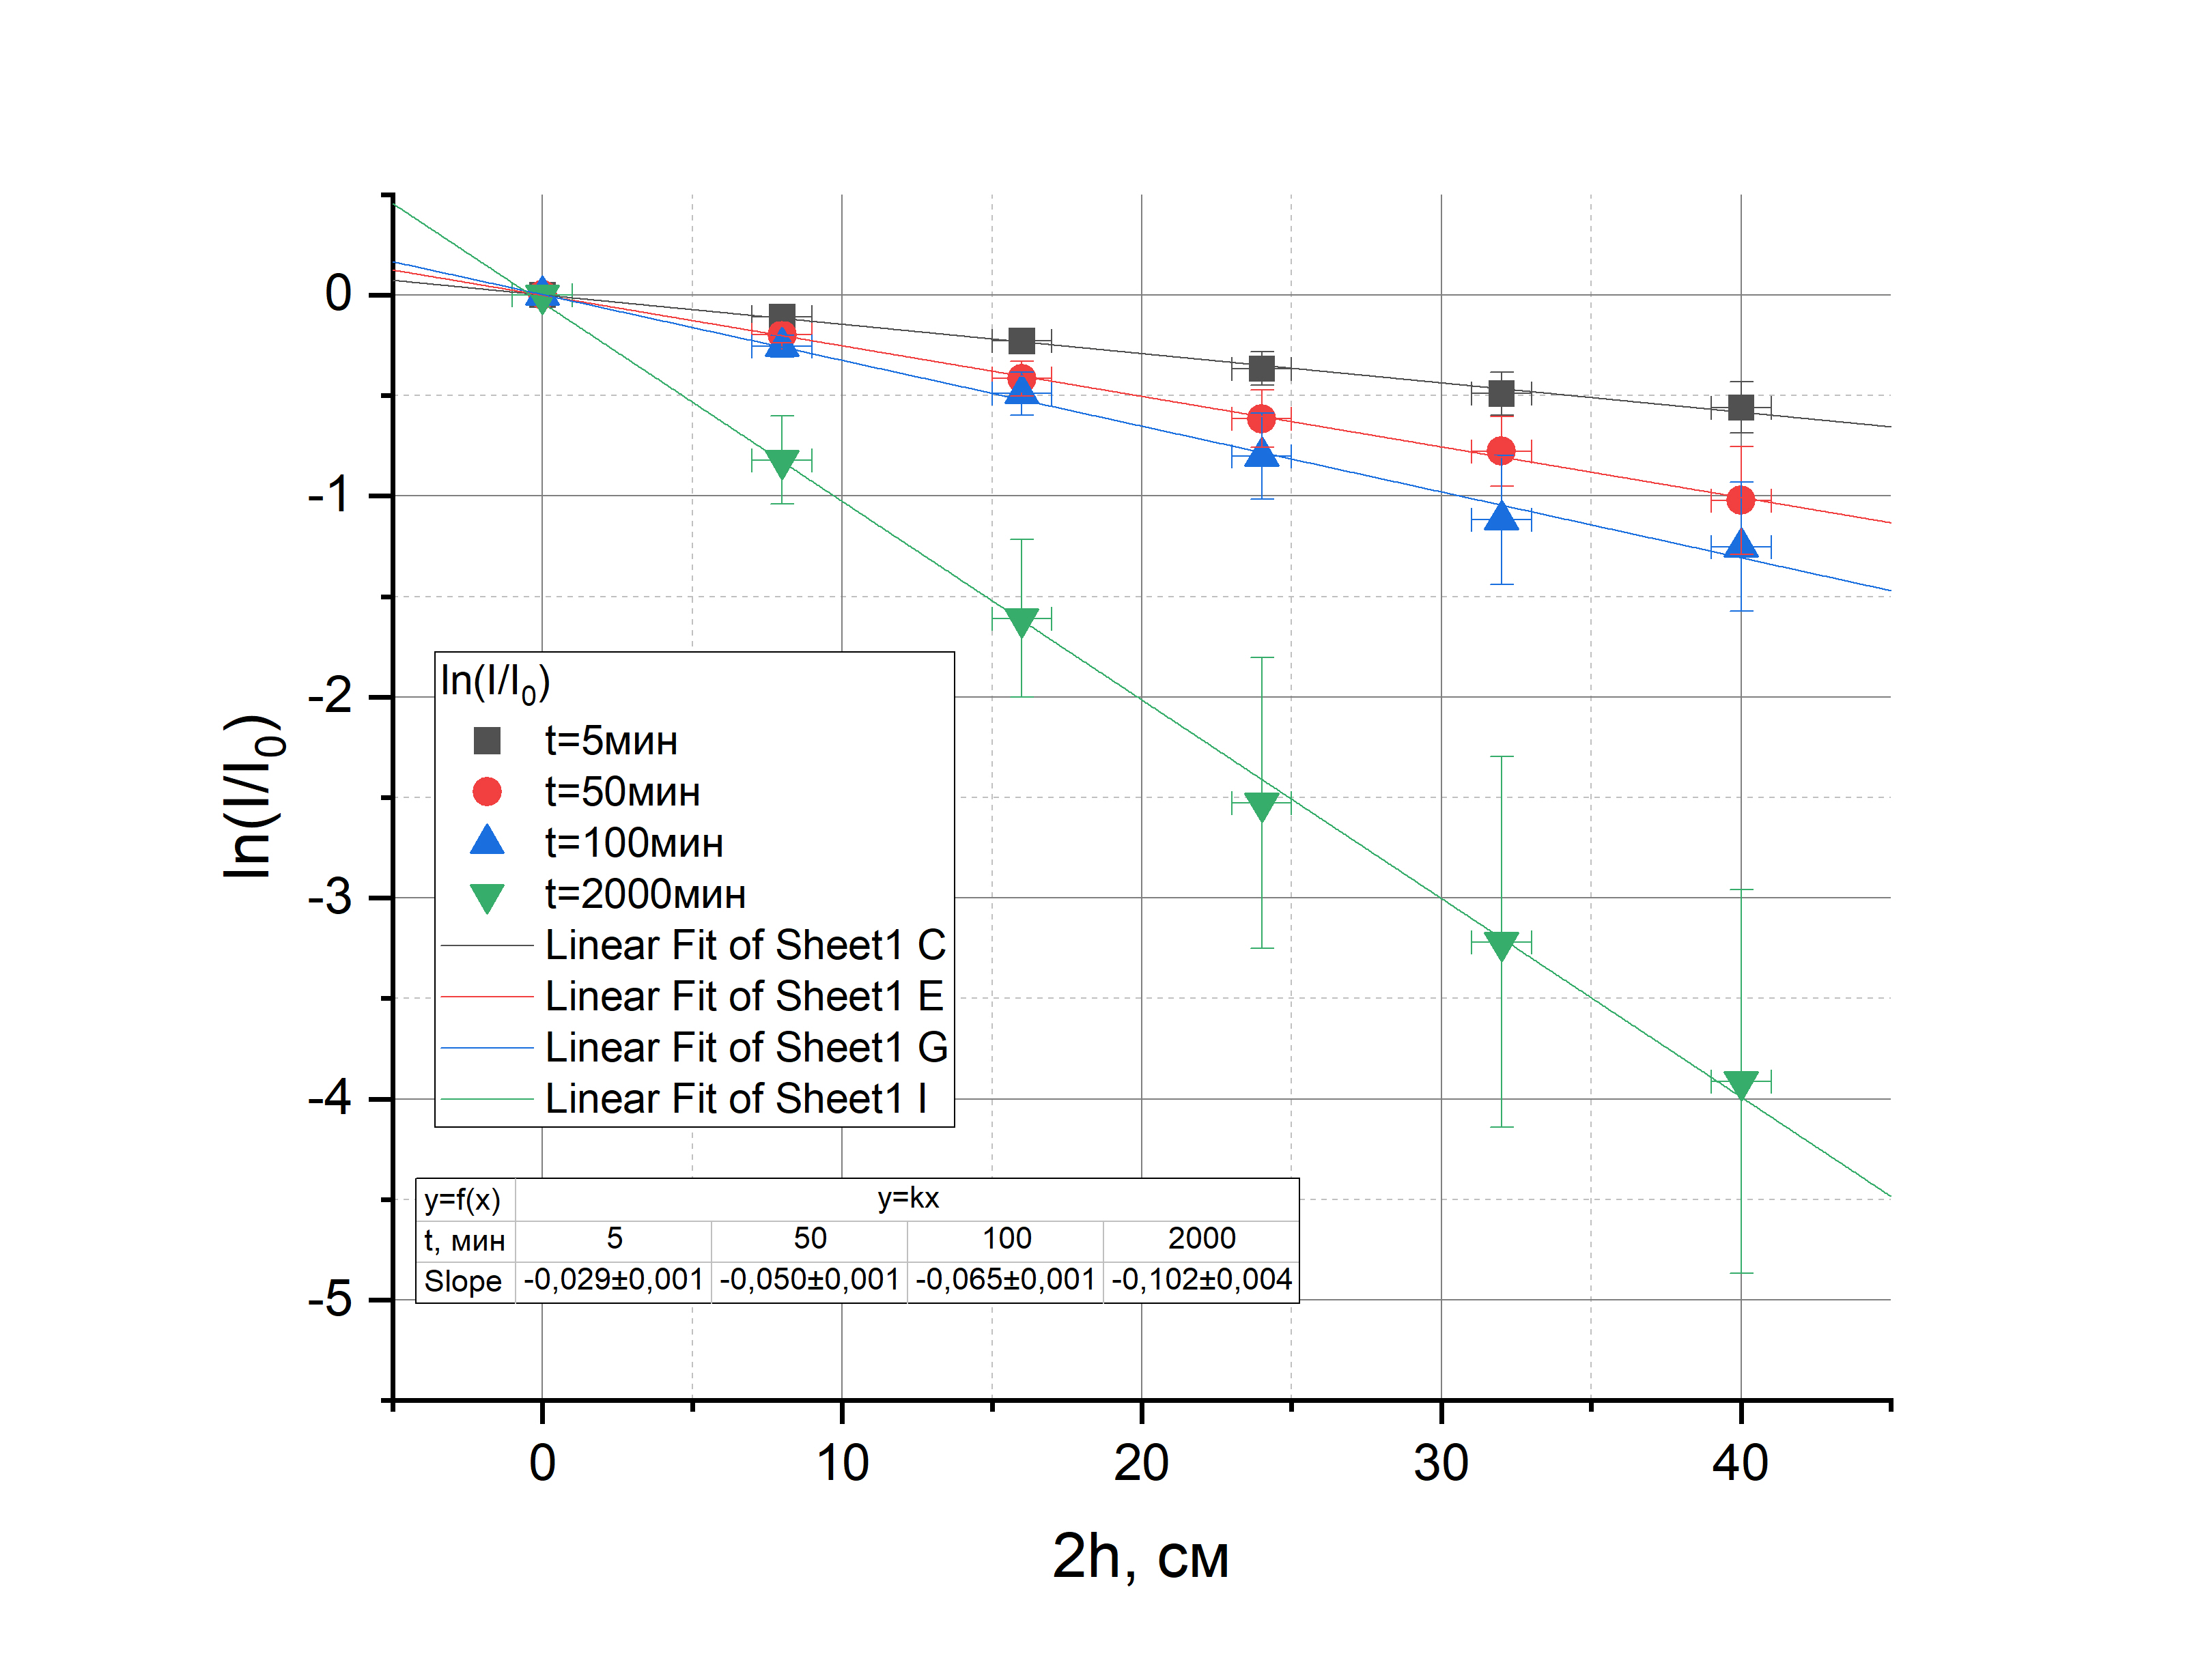
\includegraphics[width = 0.8\textwidth]{6.jpg}
\caption{Зависимость $ln(I/I_0)(2h)$ для разного времени заварки}
\end{center}
\end{figure}
В итоге получаем, что 

\begin{table}[h]
\begin{tabular}{|c|c|}
\hline
t, мин & $\alpha, \text{м}^{-1}$ \\ \hline
0      & $0,58\pm0,04$             \\ \hline
5      & $2,9\pm0,1$             \\ \hline
50     & $5\pm0,1$               \\ \hline
100    & $6,5\pm0,3$             \\ \hline
2000   & $10,2\pm0,4$            \\ \hline
\end{tabular}
\end{table}
Здесь за время 0 мы считаем, когда у нас не было чая, далее будет понятно для чего. 

Из формул 
\[dN_{\text{ф}} = - p N_{\text{ф}}dN\]
\[dI =-\alpha I dx\]
Можно получить, что 
\[\alpha = pSn\]
Очевидно, что можно принять постоянными площадь сосуда и вероятность поглощения фотона, так как жидкость однородна (из-за этого может возникнуть погрешность, поскольку легко наблюдать, что в самые первые секунды заварки чая жидкость неоднородная, и вокруг чаинок концентрация чая, а соответственно и $p$ больше, чем далеко от чаинок, на другом конце стакана, например), то 
\[n = k \alpha\]
При заваривании чая, появляются, со временем, новые молекулы, поэтому \[\alpha = \alpha_{all} - \alpha_{water} = \alpha_{tea}\]

Так же, необходимо учесть, что в самом начале, как только мы начинаем заваривать чай, у нас уже сразу часть заварена, из-за этого у нас в предполагаемой экспоненте возникает еще один коэффициент, так скажем "подгоночный"

Из этого предположения следует, что 
\[n \approx n_0 \left(1-e^{-B-At}\right)\]
Проверим это 
\begin{figure}[h]
\begin{center}
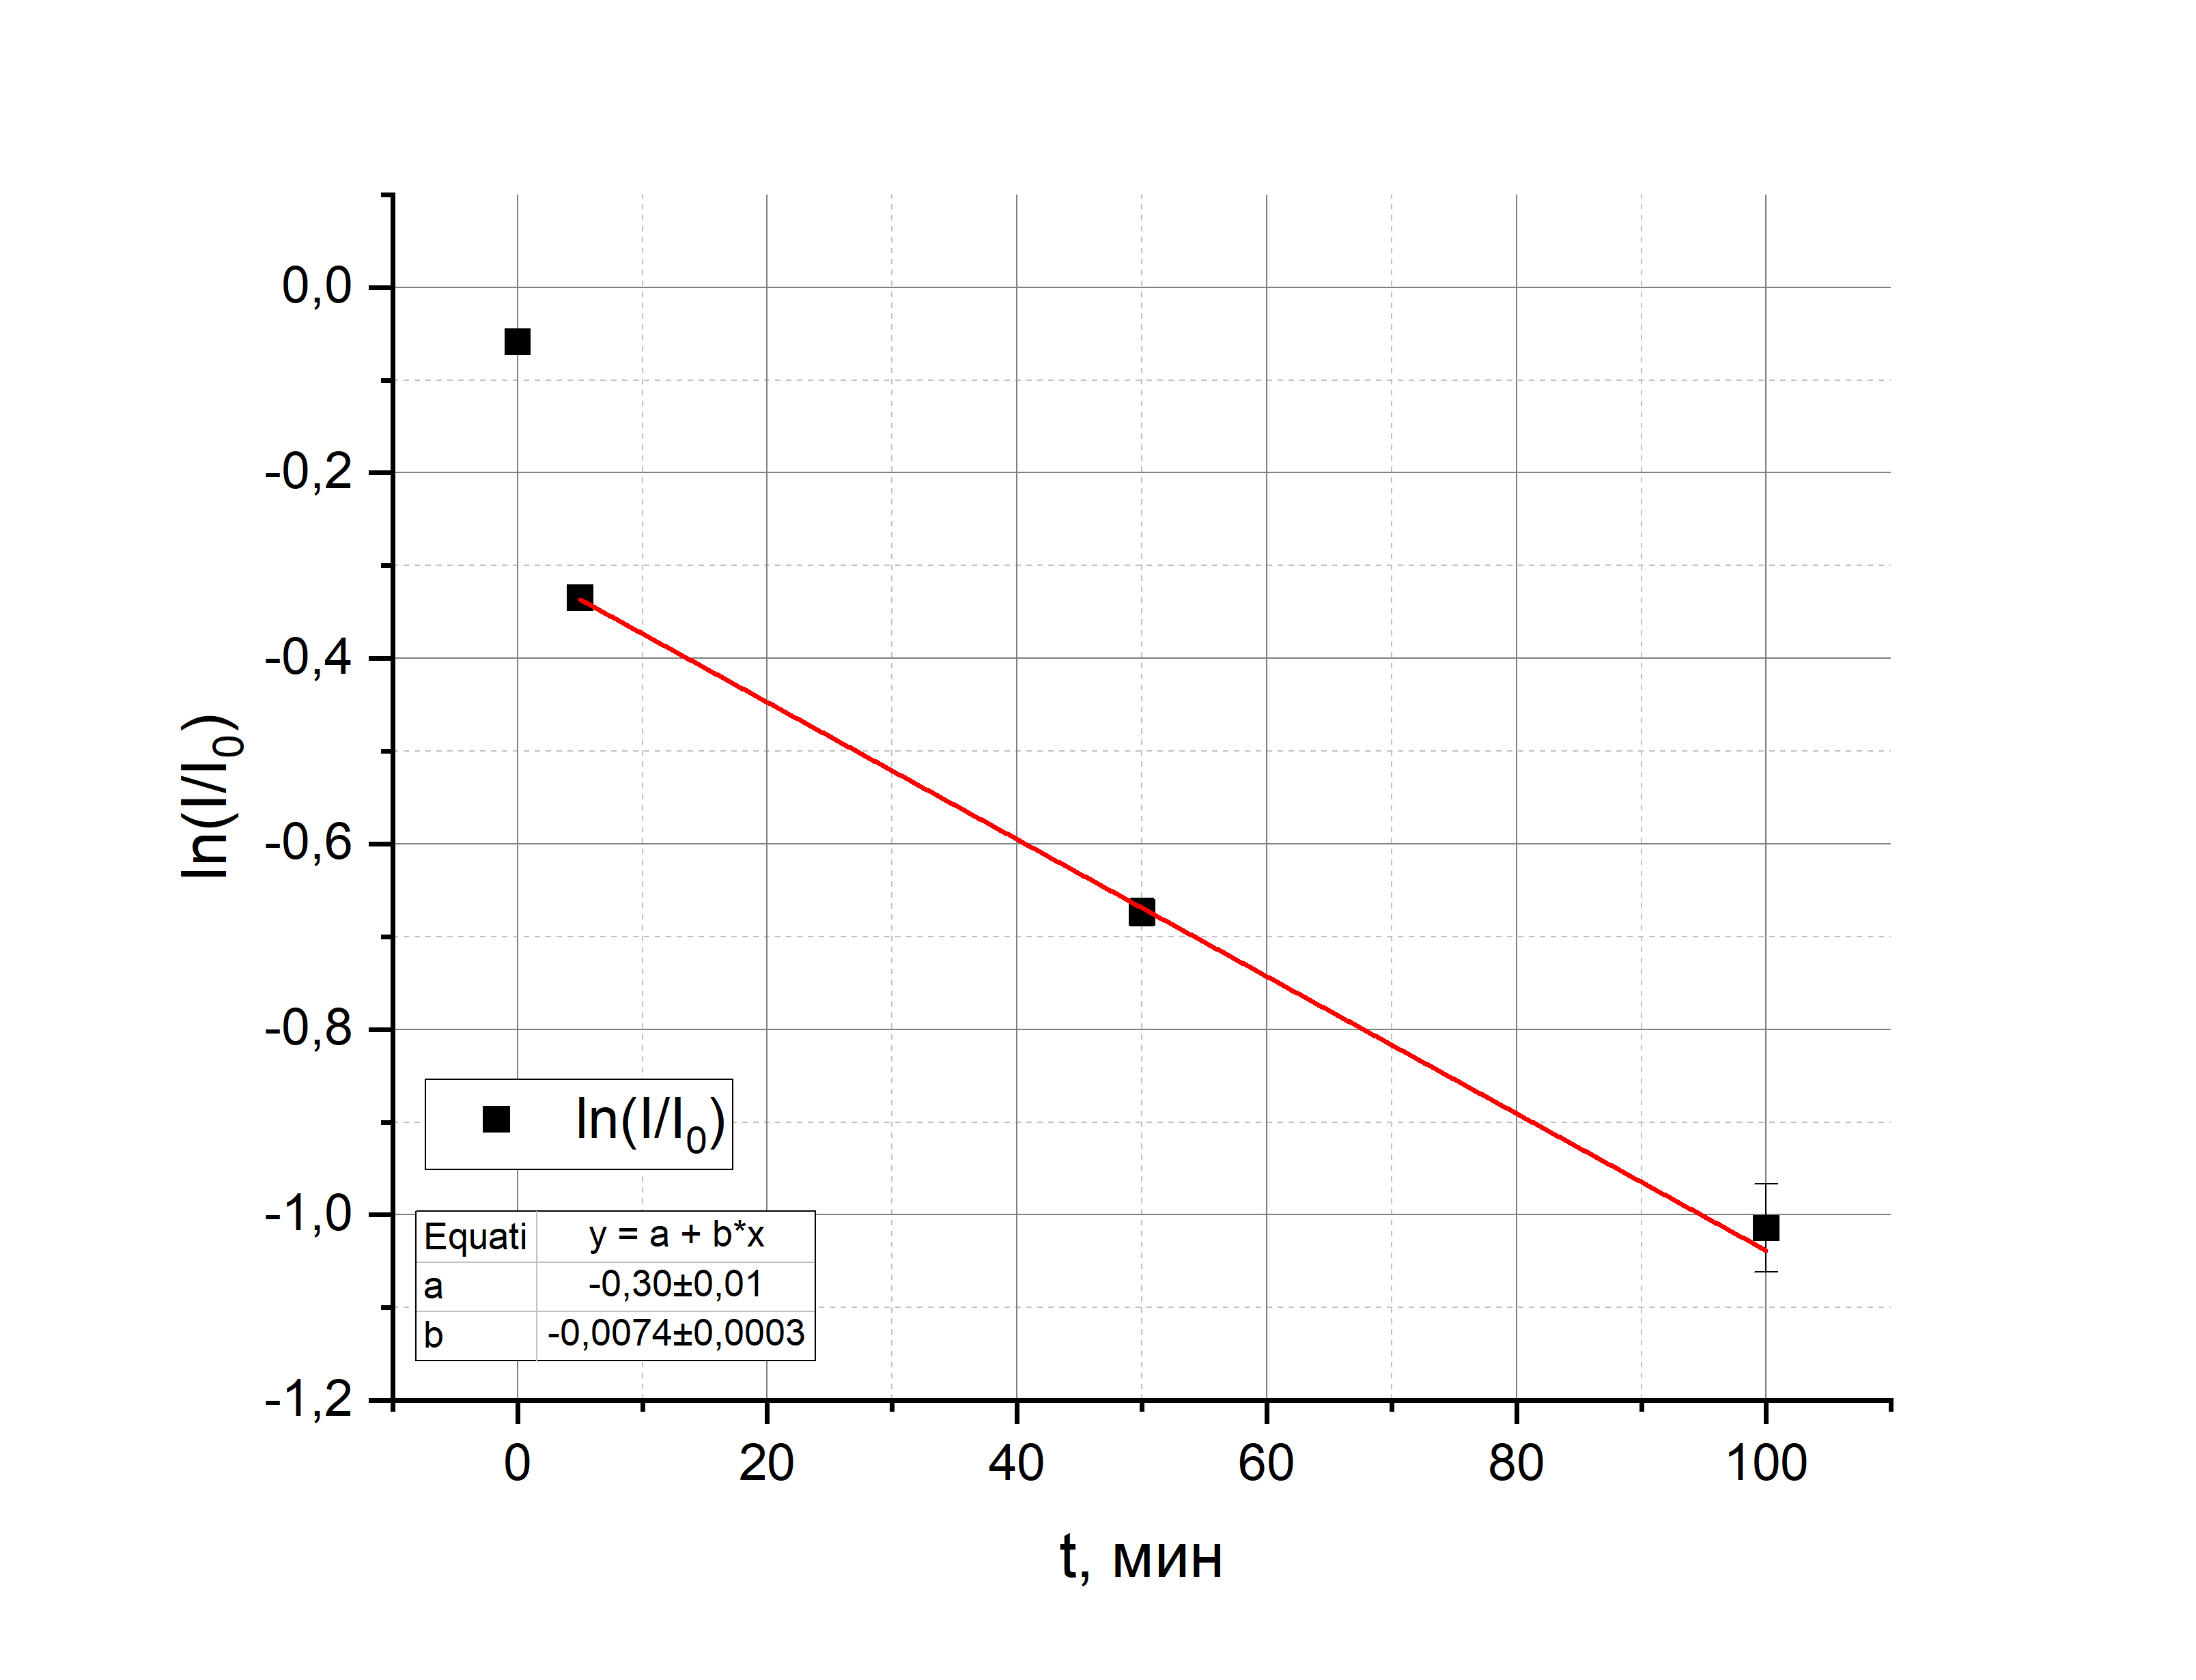
\includegraphics[width = 0.8\textwidth]{7.jpg}
\caption{Зависимость $\ln\left(\frac{\alpha_0-\alpha}{\alpha_0}\right)$}
\end{center}
\end{figure}

В графике $\alpha_0$ --- $\alpha_{tea}$, $\alpha$ --- при этом времени.

 Погрешность $\ln\left(\frac{\alpha_0-\alpha}{\alpha_0}\right)$ считаем по формуле
\[\sigma_{\ln\left(\frac{\alpha_0-\alpha}{\alpha_0}\right)} = \sqrt{\left(\frac{\sigma_{\alpha}}{\alpha_0-\alpha}\right)^2+\left(\frac{\sigma_{\alpha_0} \alpha}{\alpha_0-\alpha}\right)^2}\]
В итоге видим, что наша оценка $n(t)$ справедлива и, в итоге,
\[A = (7,4 \pm 0,3) \cdot 10^{-3} \text{мин}^{-1}\]
\[B = (0,30 \pm 0,01)\]
\section*{Вывод}
Мы удостоверились, что закон Ламберта-Бугера-Бера работает. Так же мы выяснили зависимость концентрации поглощающих веществ от времени.
\end{document}